\documentclass[12pt]{article} % use larger type; default would be 10pt
\usepackage[czech]{babel}
\usepackage[utf8]{inputenc} % set input encoding (not needed with XeLaTeX)

%%% PAGE DIMENSIONS
\usepackage{geometry} % to change the page dimensions
% \usepackage[left=2cm,right=2cm,top=2cm,bottom=2cm]{geometry}
\geometry{a4paper}
% \geometry{margin=2in} % for example, change the margins to 2 inches all round
% \geometry{landscape} % set up the page for landscape

\usepackage{graphicx} % support the \includegraphics command and options
\usepackage{wrapfig} % support the wrapfigure section

\usepackage{hyperref} % links in \tableofcontents
\hypersetup{
	colorlinks,
	citecolor=black,
	filecolor=black,
	linkcolor=black,
	urlcolor=black
}

% \usepackage[parfill]{parskip} % Activate to begin paragraphs with an empty line rather than an indent

%%% PACKAGES
\usepackage{booktabs} % for much better looking tables
\usepackage{array} % for better arrays (eg matrices) in maths
%\usepackage{paralist} % very flexible & customisable lists (eg. enumerate/itemize, etc.)
\usepackage{verbatim} % adds environment for commenting out blocks of text & for better verbatim
\usepackage{subfig} % make it possible to include more than one captioned figure/table in a single float
% These packages are all incorporated in the memoir class to one degree or another...
\usepackage{tikz} % graphs
\usepackage{pgfplots}
\usepackage{float}

%%% HEADERS & FOOTERS
\usepackage{fancyhdr} % This should be set AFTER setting up the page geometry
\pagestyle{fancy} % options: empty , plain , fancy
\renewcommand{\headrulewidth}{0pt} % customise the layout...
\lhead{}\chead{}\rhead{}
\lfoot{}\cfoot{\thepage}\rfoot{}

%%% SECTION TITLE APPEARANCE
\usepackage{sectsty}
\allsectionsfont{\sffamily\mdseries\upshape} % (See the fntguide.pdf for font help)
% (This matches ConTeXt defaults)

%%% ToC (table of contents) APPEARANCE
\usepackage[nottoc,notlof,notlot]{tocbibind} % Put the bibliography in the ToC
\usepackage[titles,subfigure]{tocloft} % Alter the style of the Table of Contents
\renewcommand{\cftsecfont}{\rmfamily\mdseries\upshape}
\renewcommand{\cftsecpagefont}{\rmfamily\mdseries\upshape} % No bold!
\newcommand{\bigsize}{\fontsize{35pt}{20pt}\selectfont}

%%% END Article customizations

\begin{document}
\begin{titlepage}
	
\includegraphics[scale=0.7]{logo.jpg}
	\vspace*{\fill}
	\begin{center}
		\textsc{\LARGE Porovnávání dvou kmitočtů a jejich odchylky}\\[1cm]
		Martin Zlámal \\[1cm]
		{\small\em \copyright \ Datum poslední revize \today } \\
		\LaTeX
	\end{center}
	\vspace*{\fill}
\end{titlepage}
%\tableofcontents
%\listoffigures
%\listoftables
\newpage

\section{Zadání}
\begin{enumerate}
\item Změřte odchylku síťového kmitočtu při poměru kmitočtů 1: 1.
\item Sledujte odchylku síťového kmitočtu během 30 min.
\item Stanovte střední hodnotu kmitočtu a velikost kolísání.
\item Pozorujte Lissajousovy obrazce pro různé poměry kmitočtů.
\end{enumerate}

\section{Teoretický úvod}
\begin{description}
\item[Osciloskop v režimu XY] \hfill \\
Osciloskop v režimu XY umožňuje prokládat dva vstupní signály na navzájem kolmou osu jejiž kompozicí získáme Lissajousovy obrazce
\item[Lissajousovy obrazce] \hfill \\
Lissajousovy obrazce jsou rovinné křivky, které vznikají skládáním dvou 
harmonických pohybů ve dvou navzájem kolmých přímkách. Tvar takovýchto křivek je 
jednoznačně zadán poměrem úhlových frekvencí a velikostí počáteční fáze $\varphi$.
\end{description}

\section{Schéma zapojení}
\begin{figure}[H]
\center
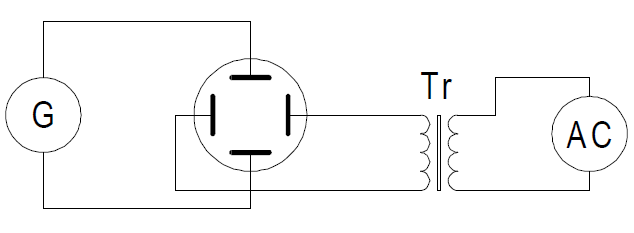
\includegraphics[scale=0.8]{schema.png}
\caption{Schéma zapojení osciloskopu}
\end{figure}

\section{Naměřené a vypočítané hodnoty}
Pro výpočet poměru kmitočtů je zapotřebí ustálit Lissajousův obrazec v uzavřeném stavu. V takovém případě jsou frekvence shodné a fázový posuv mezi nimi je $\varphi = 0$. V takovém případě poměr kmitočtů spočteme jako:
\begin{equation}
\frac{f_y}{f_x} = \frac{n_x}{n_y} \qquad \frac{100 [Hz]}{50 [Hz]} = \frac{2}{1}
\end{equation}
Jinak řečeno, pokud se na ose Y zobrazuje signál o frekvenci $100Hz$ a skládá se se signálem na ose X o frekvenci $50Hz$, potom je poměr kmitočtů 2. To se dá velmi snadno spočítat z tvaru Lissajousova obrazce, který bude mít v tomto případě vzhledem k ose X dotykové body 2 a na ose Y pouze 1. Toto obecně platí pro všechny násobky frekvencí.

Naměření časy potřebné pro změnu celého cyklu jsou (po seřazení a přepočtení na sekundy):
$30, 30, 33, 34, 44, 45, 45, 52, 57, 65, 74, 76, 87, 102, 158 [s]$. Z těchto časů snadno spočteme střední hodnotu jakožto aritmetický průběh, který se rovná $62s$. Střední hodnota kmitočtu je tedy:
\begin{equation}
\pm \Delta f = \frac{1}{T} = \frac{1}{62} = \pm 0,016Hz
\end{equation}

Velikost kolísání $k$ lze stanovit jako rozdíl největší a nejmenší odchylky, tedy:
\begin{equation}
k = \frac{1}{T_{min}} - \frac{1}{T_{max}} = \frac{1}{30} - \frac{1}{158} = 0,027Hz
\end{equation}

\section{Závěr}
Podle našeho měření vychází, že se síťový kmitočet od deklarované hodnoty $50Hz$ liší maximálně o $0,027Hz$ a to v největších extrémech. V průměru se síťový kmitočet liší pouze o $\pm 0,016Hz$. Při měření se také ukázalo, že záleží na tom, jaká a kolik zařízení je připojeno a zapnuto v síti. Zatímco při plném využívání laboratoře docházelo k odchylkám největším, při vypnutí přístrojů již byla odchylka od deklarovaného síťového kmitočtu nejmenší (až $0,0063Hz$).

\section{Přístroje}
\begin{itemize}
\item Osciloskop OS-504RD, evid. 109718
\item Generátor TR0456
\end{itemize}

\end{document}
